% Goal: One-page standalone handout of the conceptual framework (Figure 1 of the lit review)
% Andie Creel / Started November 2026
%
% Simplified from the tikzpicture in manuscript/main.tex (fig:cascade): no examples, definitions inside the boxes.

\documentclass[12pt]{article}

% Language setting
\usepackage[english]{babel}

% Set page size and margins (landscape so the wide figure can be larger)
\usepackage[letterpaper,landscape,top=2cm,bottom=2cm,left=2.5cm,right=2.5cm]{geometry}

% Useful packages
\usepackage{graphicx}
\usepackage{tikz}
\usetikzlibrary{arrows.meta, decorations.pathreplacing, positioning}
\usepackage{natbib}
\usepackage{xurl} % lets long URLs in the bibliography break across lines
\usepackage{array} % m{} columns: vertically centered table cells
\usepackage{enumitem} % compact bulleted lists inside the table cells
\usepackage[colorlinks=true, allcolors=blue]{hyperref}

\pagestyle{empty}

% Bulleted lists inside the table cells
\setlist[itemize,1]{label=\textbullet, leftmargin=5em} % one extra indent (table cells override this with cellitems)
\setlist[itemize,2]{label=$\circ$} % hollow sub-bullets
\SetEnumitemKey{cellitems}{leftmargin=1.6em, topsep=0pt, partopsep=0pt, itemsep=1pt, parsep=0pt, before=\vspace{11pt}, after=\vspace{8pt}}

\begin{document}

\begin{center}
{\Large \textbf{Three Key Terms Regarding Ecosystem Services}}\\[0.4em]
Andie M. Creel \\ \today
\end{center}

\vspace{1em}

% ------------------------------------------------------------------------------
% Conceptual framework
% ------------------------------------------------------------------------------
\begin{center}
\resizebox{0.95\linewidth}{!}{%
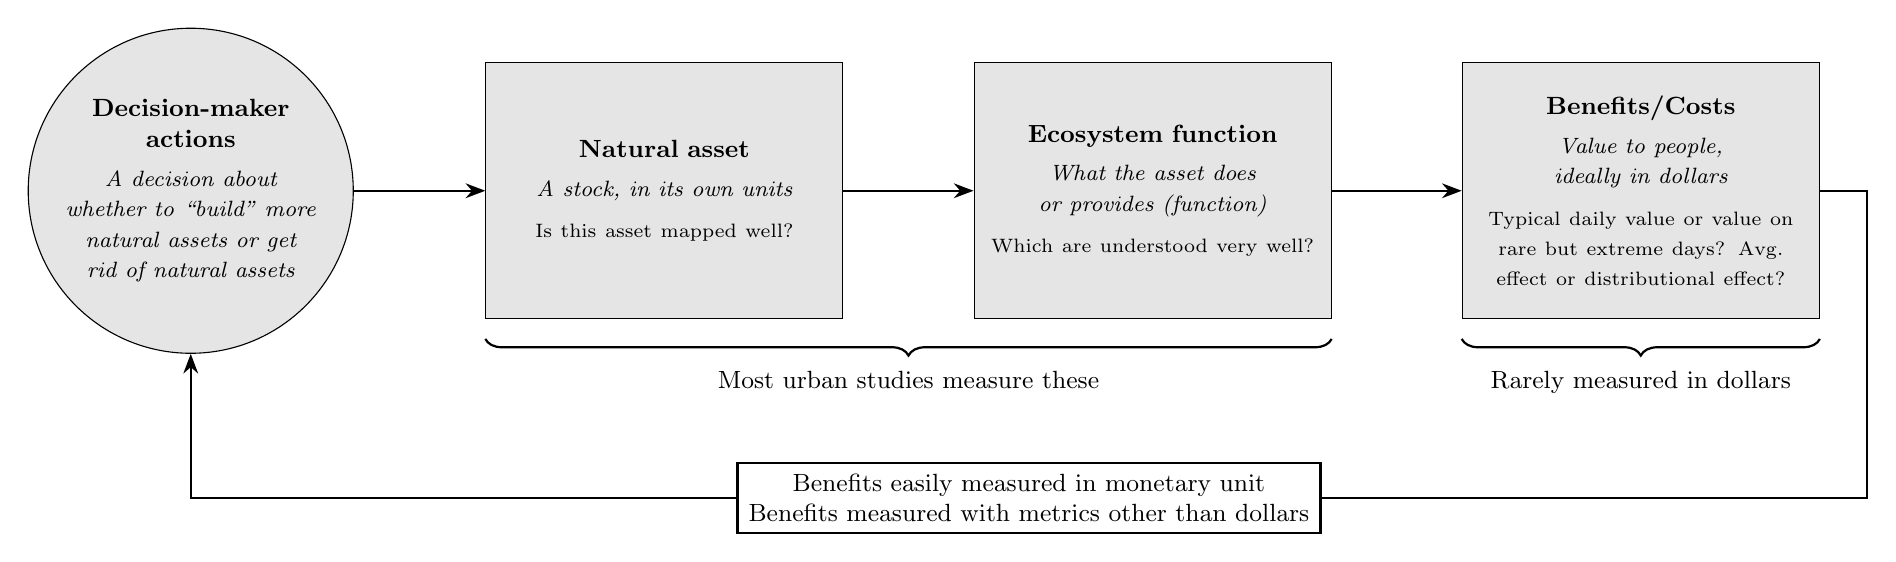
\begin{tikzpicture}[
  font=\small,
  head/.style={draw, fill=gray!20, text width=4.3cm, minimum height=3.25cm, align=center},
  arr/.style={-{Stealth[length=2.5mm]}, thick}
]
  % Boxes: term in bold, definition in italics
  \node[head] (a) at (0,0)    {\textbf{Natural asset}\\[3pt]{\footnotesize\itshape A stock, in its own units}\\[4pt]{\scriptsize Is this asset mapped well?}};
  % Circle: decision-maker actions
  \node[circle, draw, fill=gray!20, text width=3.3cm, align=center, inner sep=1pt] (d) [left=1.67cm of a]
    {\textbf{Decision-maker}\\\textbf{actions}\\[3pt]{\footnotesize\itshape A decision about whether to ``build'' more natural assets or get rid of natural assets}};
  \draw[arr] (d) -- (a);
  \node[head] (s) at (6.2,0)  {\textbf{Ecosystem function}\\[3pt]{\footnotesize\itshape What the asset does or provides (function)}\\[4pt]{\scriptsize Which are understood very well?}};
  \node[head] (b) at (12.4,0) {\textbf{Benefits/Costs}\\[3pt]{\footnotesize\itshape Value to people, ideally in dollars}\\[4pt]{\scriptsize Typical daily value or value on rare but extreme days? Avg. effect or distributional effect?}};
  \draw[arr] (a) -- (s);
  \draw[arr] (s) -- (b);
  % Where the literature is
  \draw[decorate, decoration={brace, mirror, amplitude=6pt}, thick]
    ([yshift=-0.25cm]a.west |- b.south) -- ([yshift=-0.25cm]s.east |- b.south) node[midway, below=8pt] {Most urban studies measure these};
  \draw[decorate, decoration={brace, mirror, amplitude=6pt}, thick]
    ([yshift=-0.25cm]b.south west) -- ([yshift=-0.25cm]b.south east) node[midway, below=8pt] {Rarely measured in dollars};
  % Feedback arrow from benefits back to decision-makers (one arrow, both kinds of benefits)
  \draw[arr] (b.east) -- ++(0.6,0) -- ++(0,-3.9) -| node[pos=0.25, draw, fill=white, inner sep=4pt, align=center]
    {Benefits easily measured in monetary unit\\Benefits measured with metrics other than dollars} (d.south);
\end{tikzpicture}%
}
\end{center}

\vspace{1em}
\begin{center}
\begin{minipage}[t]{0.85\linewidth}
\small \noindent
\end{minipage}
\end{center}



\subsection*{Way to value benefits}
\begin{itemize}
  \item Direct use (requires you being near/visiting) versus effects you don't need to be close for
  \item Monetized units versus other metrics to well-being
\end{itemize}

\subsection*{Who is the decision maker?}
\begin{itemize}
  \item Local government
  \item National government
  \item Private sector
  \begin{itemize}
    \item Insurance companies
    \item Storefronts 
    \item Real estate developers
  \end{itemize}
  \item Non-governmental organizations
  \item Home-owners/Neighborhoods 
\end{itemize}

\subsection*{What is the decision maker's objective function?}
\begin{itemize}
  \item Minimize social disruption 
  \begin{itemize}
    \item Sectors (e.g., transportation, housing, energy, business)
    \item Social groups (e.g., race, income)
  \end{itemize}
  \item Minimize cost
  \begin{itemize}
    \item Energy cost
    \item Healthcare cost
  \end{itemize}
  \item Maximize welfare
  \begin{itemize}
    \item Recreation
    \item Spiritual/Cultural well-being
  \end{itemize}
  \item \textbf{Cities want to know the cost of doing nothing -- that is the relevant counterfactual }
  
\end{itemize}
  


\vfill
\noindent\begin{minipage}{\linewidth}
% \renewcommand{\refname}{\normalsize References}
% \footnotesize
% \bibliographystyle{aer}
% \bibliography{../references}
\end{minipage}

\end{document}
